\section[Motivation]{Motivation and History}
\subsection{Handwriting}
{\usebackgroundtemplate{%
    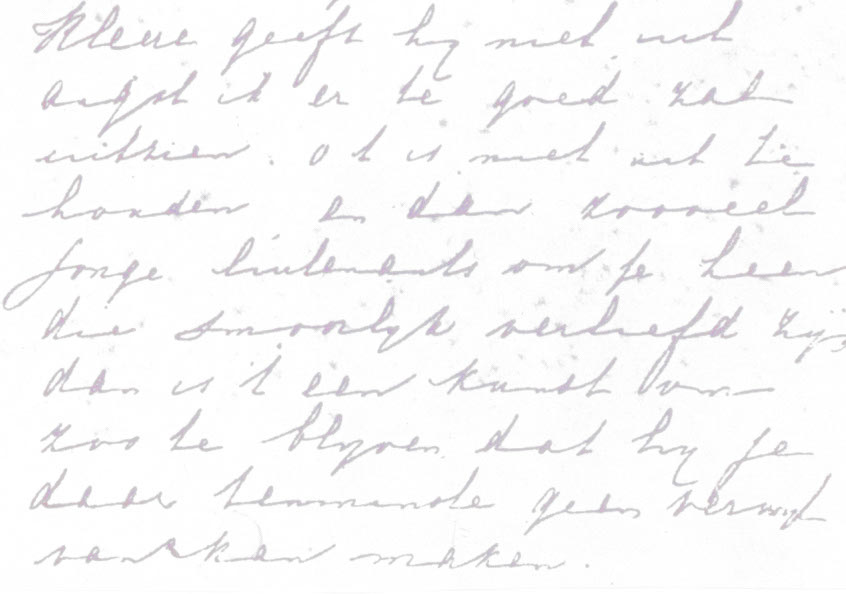
\includegraphics[width=\paperwidth,height=\paperheight]{figures/handwriting063-covered.jpg}}
  \begin{frame}{No one can write properly these days\ldots}
    \begin{itemize}
    \item Proper and beautiful writing with a quill was once an art with
      much appreciation.
    \item Nowadays you can even teach without having a proper handwriting.
      \begin{itemize}
      \item Living proof is in front of you\ldots
      \end{itemize}

    \item So who am I to expect my students to have a proper hand in writing?

    \item Note: using a pencil and paper~\footnote{White board, whatever} to make a sketch before you start
      writing/coding, even if you throw the sketch away in the process is
      still a best practice.
    \end{itemize}

  \end{frame}
}

\subsection[Use an IDE]{Use Netbeans IDE}
\begin{frame}{In practice you use an IDE}
  \begin{itemize}
  \item I have seen the days of punch cards and paper tape.
  \item Programming was programming in the small. (As was examination).
  \item Nowadays you let students use an IDE during their practical work
    \begin{itemize}
    \item For didactic purposes: You can play with the things you
      make. e.g. For Java: bluej or greenfoot.
    \item To enhance productivity, get bigger jobs done: \Okis{Netbeans IDE}.
    \item Advantage of Netbeans: pure java, runs on everything (even
      \Okis{Raspberry Pi})
    \end{itemize}
  \item Nowadays programming is programming in the large, know and
    understand the important APIs and how to use them. Read (java)doc etc.
  \item Logical consequence: Use and IDE (any of the above) during
    exams too.
  \end{itemize}
\end{frame}

\subsection[Authenticity]{Authenticity is paramount in exams}
\begin{frame}{Authenticity, Logistics, tooling}
  \begin{itemize}
  \item Examination requires certain conditions.
    \begin{itemize}
    \item Students are not allowed to share work (cheating), where in lab hours
      they are advised to do so.
    \item Only certain resources or references are allowed, where as
      in lab hours \Okis{google} and \alert{stack overflow} are available.
    \item \Okis{Solution} computers that are controlled by the examiner and
      are isolated in a examination network.
    \end{itemize}
  \item Logistics: How to collect the exam work?
    \begin{itemize}
    \item Students must be able hand in, but need to stay isolated from one another.
    \item Collecting the work from the workstations?

    \item Use a upload facility: student private repository hosted on
      a server in the examination network.
    \end{itemize}
  \end{itemize}
\end{frame}

\subsection[Repository]{Use a repository as logic tool for SE students}
\begin{frame}{From CVS to USB}
  And all in between.
  \begin{description}[short]
  \item[2005] The beginning.
    \begin{itemize}
    \item Labs with a computer per student during exam sessions.
    \item Multiboot workstations in lab. Separate exam 
      partition/os. Restricted shell (rbash). Linux (SuSE) based.
    \item Repository: \Okis{CVS} server on one workstation in the same lab.
    \item Students where well versed (well, almost) in CVS.
    \end{itemize}
  \item[2009] Moved subversion.
  \item[2012] Bring your own device.
    \begin{itemize}
    \item Mix of lab PCs and laptops. How to control the laptop during exam?
    \item Boot from USB stick.
    \item Still using a repository.
    \end{itemize}
  \item[2015] Dropped repository. Collect exam from sticks.
  \end{description}
\end{frame}

\subsection[Lessons]{Lessons Learned}
\begin{frame}{Lessons learned}
  \begin{itemize}
  \item An exam is not exam without proper surveillance or logging; it
    is a lab session at best. Consider:
    \begin{itemize}
    \item How to prevent students to collaborate?
    \item Or share exam credentials?
    \item Or booting something else then the proper exam setup?
    \item Accessing local disk, network at non allowed places?
    \end{itemize}
  \item Personally I never value or grade work handed without some
    proof of authenticity. Of course feedback still applies.
  \end{itemize}
\end{frame}

\subsection[Flash]{Flash memory is cheap}
\begin{frame}{Moore's law to the rescue}
  
  \begin{itemize}
  \item Dropping prices of USB storage make things affordable.
    \begin{itemize}
    \item Required storage space on USB stick: less then 4GB,
      including storage for user workspace/home dir.
    \item \euro 3.34 (2015-02-10) for 4GB.
    \end{itemize}
  \end{itemize}
  \begin{columns}
    \begin{column}{.65\textwidth}
      \begin{itemize}
      \item Speed up, USB 3.0 is a big productivity boost.
        \begin{itemize}
        \item Lowest capacity usable and available 16GB.
        \item Price is about 5 fold. Speed is 10 fold.
        \item Good experience with \Okis{Sandisk 16GB Extreme USB 3.0.}
        \end{itemize}
      \end{itemize}
    \end{column}
    \begin{column}{.35\textwidth}
      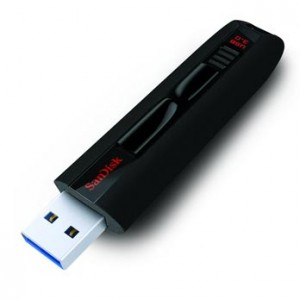
\includegraphics[width=\textwidth]{figures/SDCZ80-300x300.jpg}
    \end{column}
  \end{columns}
  \begin{itemize}
  \item Use of fitting USB hubs also works.
  \item 7 port ANKER USB 3.0 hub gives good results. 
  \end{itemize}
\end{frame}

\begin{frame}{Parallel programming, differently}
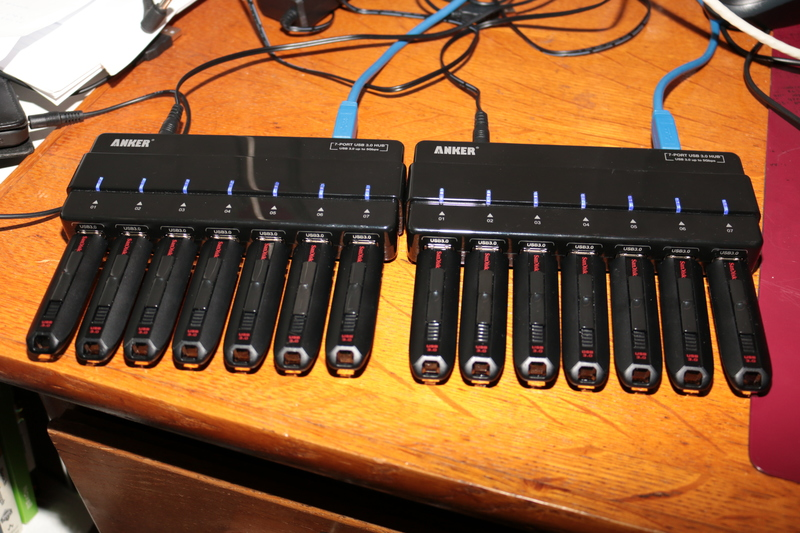
\includegraphics[width=\textwidth]{figures/14usbsticks.jpg}

\end{frame}

\begin{frame}{Other resources: 100 USB sticks}
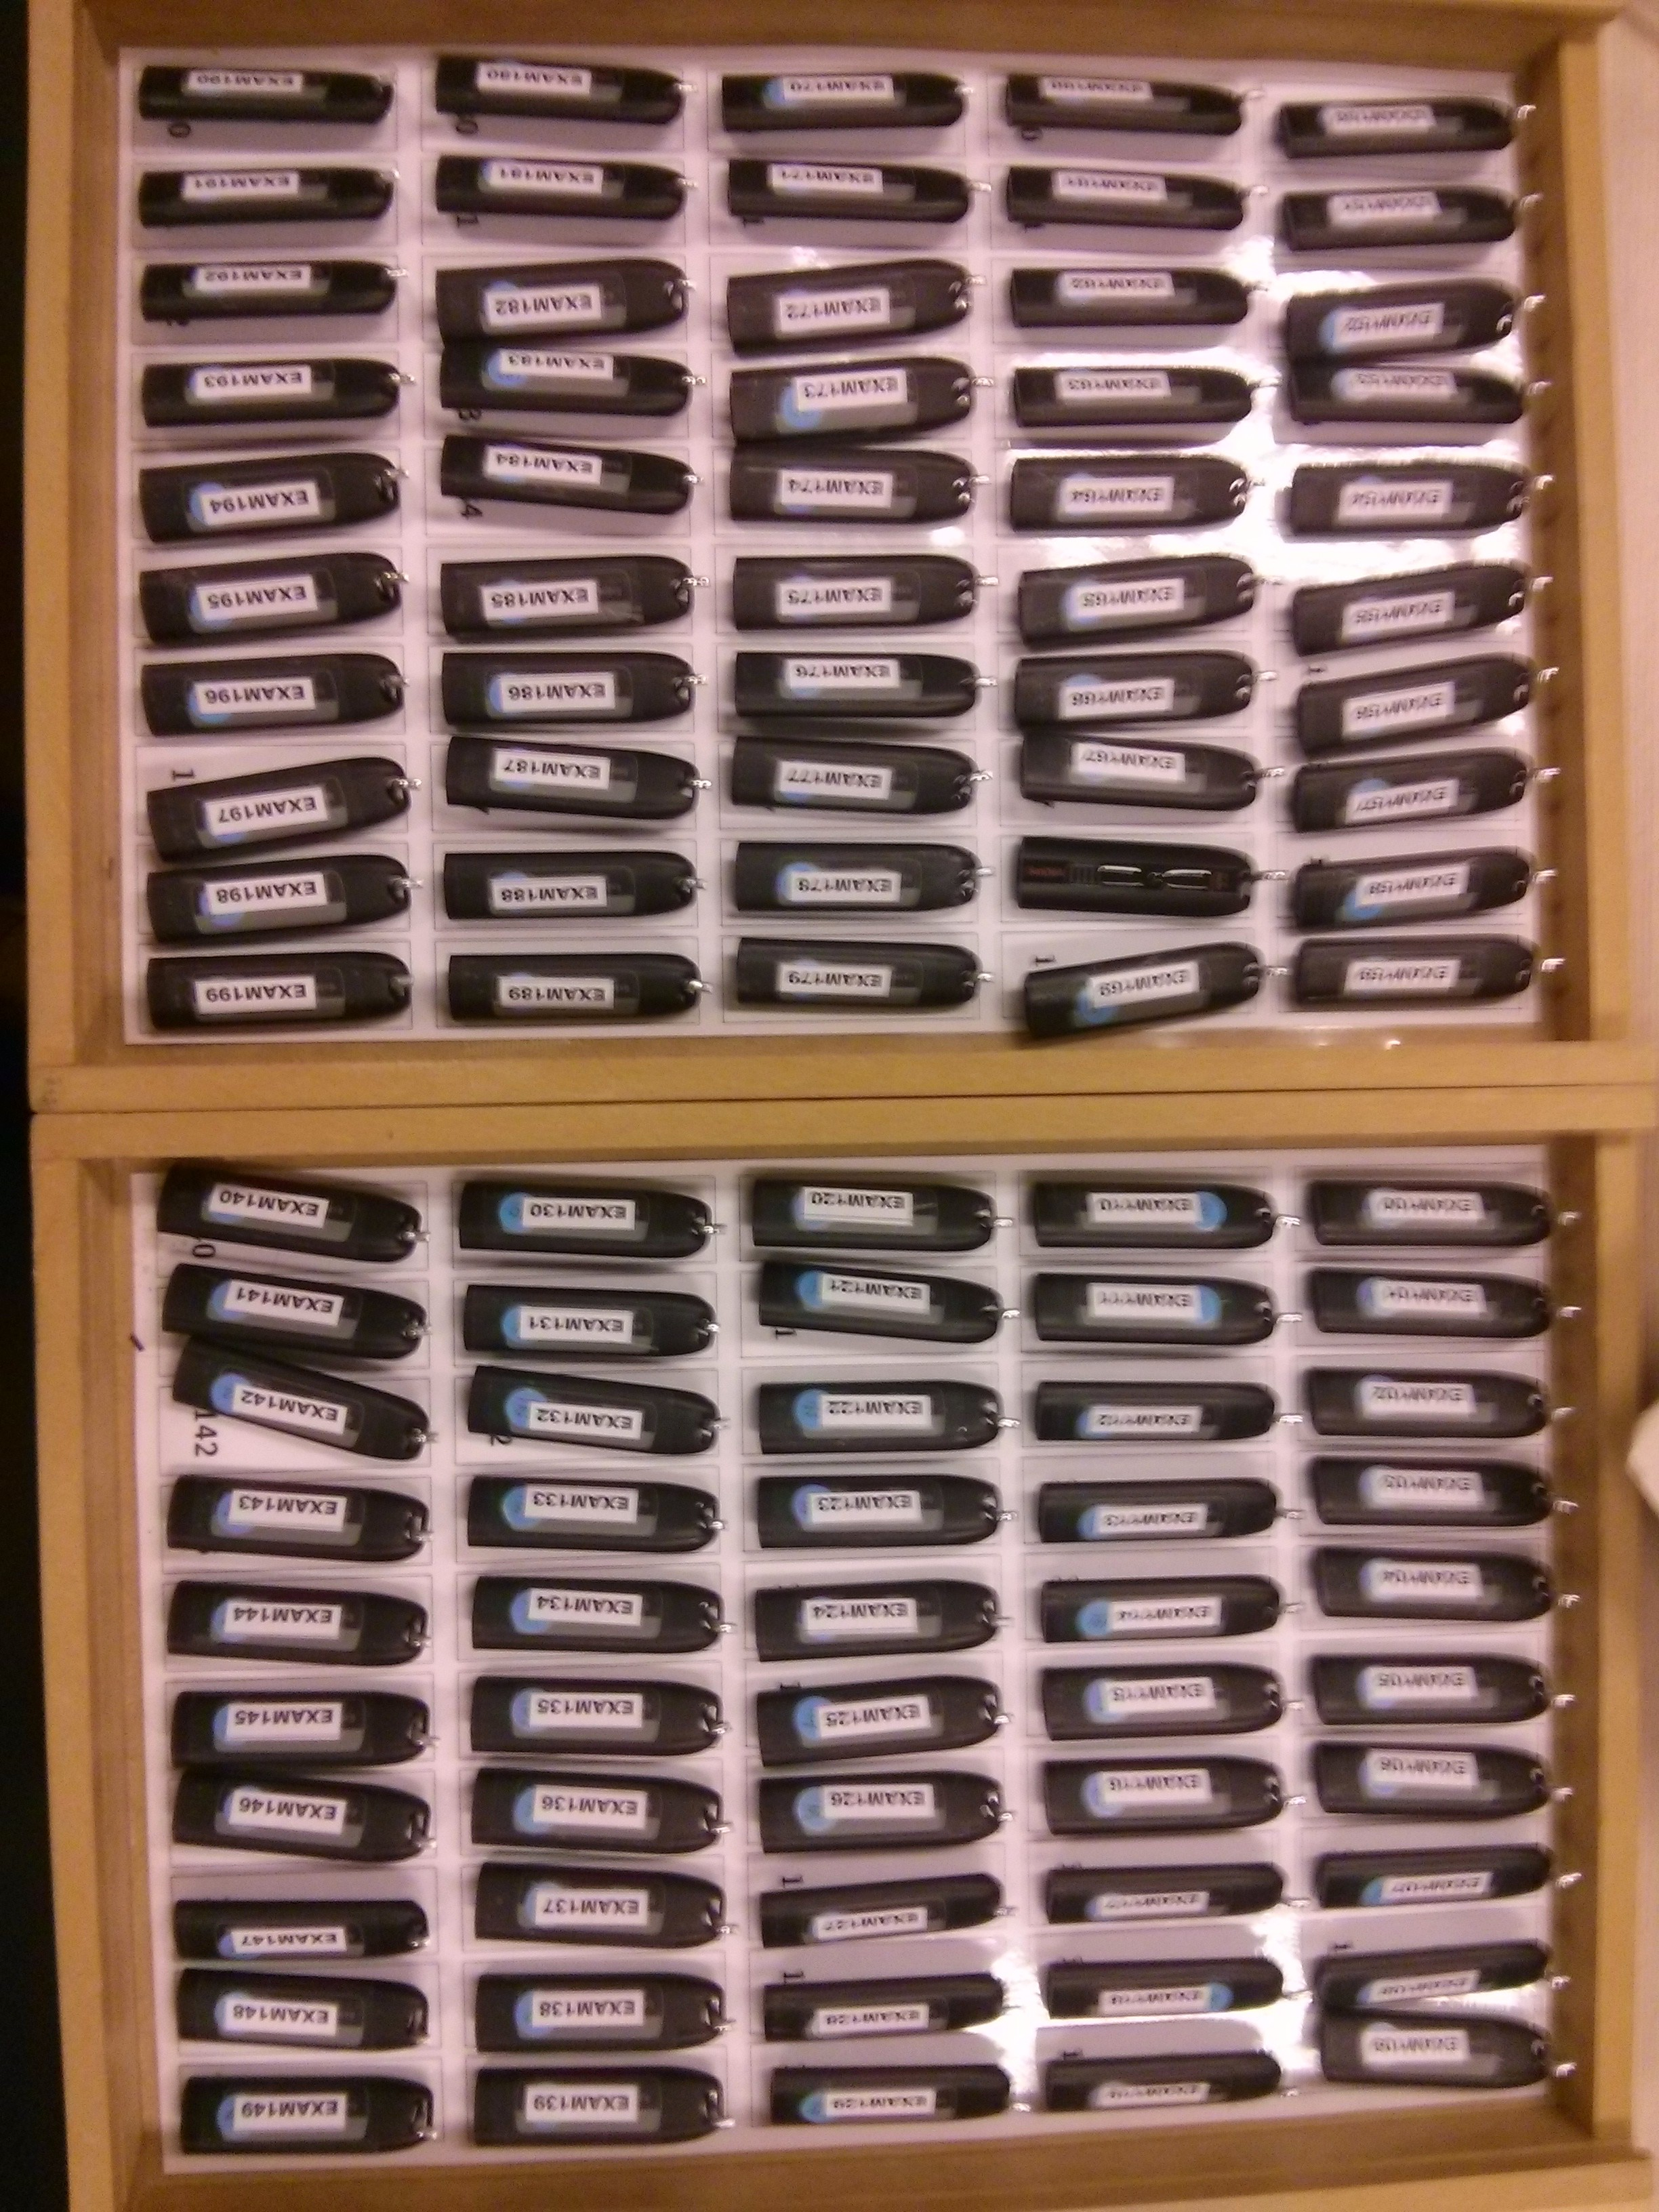
\includegraphics[angle=90,width=\textwidth]{figures/boxesofsticks.jpg}

It still amounts to about \euro 1600,-- of flash drive.
\end{frame}
